% Session 2 -- symmetry eigenstates on a ring: the phase winds.
% Placement: sec. "Worked exercises", at the three-site ring / eq. (2.4).
% Rendered by figures/blender/s02f01_ringmodes.py, labels in figures/overlays/s02f01_ringmodes.tex.
\begin{aqmfigure}{fig:s02:ring}{Symmetry fixes the eigenstates before we write down the Hamiltonian.
On a three-site ring the rotation $R$ can only have eigenvalues $e^{2\pi i n/3}$ by (2.4), and so
the coefficients of the state must change by this same phase from one site to the next. This means
that the eigenstates are the discrete Fourier modes, for any values of the hopping amplitudes. The
arrow on each site is the complex coefficient $\alpha_j\propto e^{i\varphi_n j}$, which turns by
$2\pi n/3$ from one site to the next. On the right, the balls are the allowed phases for $L=3$ and
$L=5$. In the limit $L\to\infty$ they fill the circle, and this circle is the first Brillouin zone.}
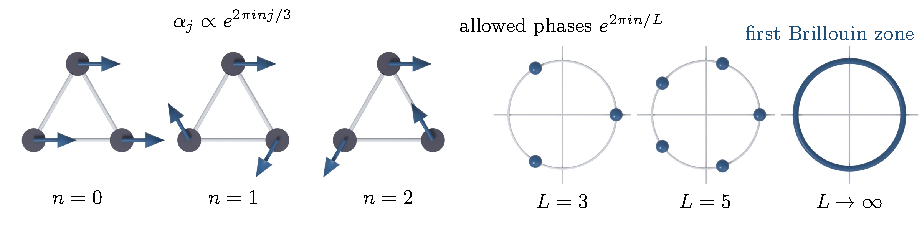
\includegraphics{figures/pdf/s02f01_ringmodes.pdf}
\end{aqmfigure}
